\documentclass[preprint,12pt,authoryear]{elsarticle}

\usepackage{amsmath,amssymb,amsfonts,amsthm}
\usepackage{booktabs}
\usepackage{tabularx}
\usepackage{graphicx}
\usepackage{natbib}
\usepackage{hyperref}
\usepackage{geometry}
\usepackage{caption}
\usepackage{subcaption}
\usepackage{float}

\geometry{a4paper, margin=1in}

\journal{Ecological Economics}

\begin{document}

\begin{frontmatter}

\title{Empirical Case Study: Real-World Pricing and RRP/D Fairness Audit --- Food, Fuel, Energy, and Shelter Materials}

\author{Jarrod Lyndsay Hamilton}
\address{Alethekanon Research Institute, Division 2: Societal Economics \& Macro-Micro Simulation, Australia}

\begin{abstract}
Neoclassical microeconomic doctrine treats market price as an unobservable, subjective equilibrium scalar ($P = f(S, D)$), asserting that prices reflect voluntary marginal utility and symmetrical competitive market clearing. This paper presents a complete empirical operationalization of the Universal Price Equation (UPE) from Value Physics, constructing forward biophysical prices and reverse-engineering observed commercial Recommended Retail Prices (RRP) across fourteen foundational necessities spanning six essential sectors in eastern Australia: Food, Agriculture, Liquid Fuels, Power Utilities, Municipal Water/Sanitation, Essential Healthcare, Building Materials, and Spatial Freight Logistics. Drawing on official empirical microdata from ABARES, the Australian Bureau of Statistics (ABS), the Australian Energy Market Operator (AEMO), the Australian Competition and Consumer Commission (ACCC), the National Heavy Vehicle Regulator (NHVR), and regional local government authorities, we decompose each price into its physical substrate base ($P_b$), thermodynamic exergy destruction ($P_e$), and human metabolic labor difficulty ($U$, measured in WEST tokens). Solving the inverse UPE for the implied institutional extractive drag fraction ($R_a$), we establish an objective, non-usurious Recommended Retail Price based on Difficulty (RRP/D). The empirical findings demonstrate that market prices embed an institutional extractive drag ($R_a$) ranging from 20.8\% in owner-operator municipal water cartage up to 59.1\% in corporate road freight logistics, establishing that cost-of-living inflation across Australia's core provisioning supply chains is fundamentally an institutional rentier extraction pathology rather than a failure of physical worker productivity.
\end{abstract}

\begin{keyword}
Universal Price Equation \sep Value Physics \sep Recommended Retail Price based on Difficulty (RRP/D) \sep Extractive Drag \sep Biophysical Economics \sep Cambridge Capital Controversy
\JEL D43 \sep L11 \sep Q01 \sep Q40 \sep R41
\end{keyword}

\end{frontmatter}

\section{Introduction \& Epistemological Critique of Subjective Pricing}
Standard neoclassical microeconomic doctrine asserts that market price represents the marginal utility of consumers balanced against the marginal cost of production. In this paradigm, prices serve as costless information vectors guiding optimal resource allocation. However, this framework suffers from three fatal physical and institutional blind spots:
\begin{enumerate}
    \item \textbf{Dimensional Incommensurability:} Neoclassical production functions treat capital, energy, and labor as fungible value aggregates denominated in nominal currency, ignoring the thermodynamic reality that physical goods require irreversible exergy destruction \citep{georgescu1971entropy} and finite human metabolic work.
    \item \textbf{Coercive Asymmetry:} Consumers purchasing essential subsistence goods (such as potable water, staple grain, domestic heating, or shelter materials) face severe biological and legal penalties if they refuse transactions. Market exchanges under existential necessity are coercive rather than Pareto-optimal.
    \item \textbf{Institutional Rent Extraction:} Corporate oligopolies, financialized intermediaries, and speculative gatekeepers levy substantial tollbooth rents that inflate retail prices far above actual thermodynamic and metabolic reproduction costs \citep{soddy1926wealth, sraffa1960production}.
\end{enumerate}

Value Physics resolves these pathologies by replacing subjective utility with the \textbf{Universal Price Equation (UPE)} \citep{hamilton2026vpe21, hamilton2026vpe49}, anchoring economic valuation in physical thermodynamics, ecological regeneration rates, and biological human exertion.

\section{Mathematical Architecture: Forward Pricing vs. Reverse RRP Dissection}

\subsection{The Universal Price Equation (UPE)}
The Universal Price Equation models price as an explicit tri-layer biophysical tensor:
\begin{equation}
P = m_1 \cdot m_2 \cdot \gamma(v_{\text{rel}}) \cdot \left[ \frac{S \cdot U}{R_n (1 - R_a)} \right] + P_e + P_b
\label{eq:upe}
\end{equation}
where:
\begin{itemize}
    \item $P_e$ (\textbf{Thermodynamic Exergy Base}): Direct thermodynamic energy consumed and destroyed in transformation, heat, electricity, and haulage (Joules, kWh, or diesel litres converted to local currency equivalents).
    \item $P_b$ (\textbf{Physical Material Base}): Sunk non-energy raw material mass, seed, fertilizer, mineral substrate, and capital replacement depreciation.
    \item $U$ (\textbf{Metabolic Labor Difficulty}): Human biological work, cognitive attention, and operational skill, quantified in standard WEST Difficulty Tokens (1 WEST $\approx$ baseline metabolic person-hour normalized to local living wage parity).
    \item $S$ (\textbf{Local Scarcity Multiplier}, $S \ge 1.0$): Regional supply constraint or storage buffer deficit factor.
    \item $R_n$ (\textbf{Environmental Regeneration Capacity}, $0 < R_n \le 1.0$): Replenishment rate of the ecological or mineral substrate (e.g., pasture regrowth, crop cycles, aquifer recharge).
    \item $R_a$ (\textbf{Institutional Extractive Drag Fraction}, $0 \le R_a < 1.0$): Unearned speculative rent, financialized interest overhead, and monopolistic margin tolls.
    \item $\gamma(v_{\text{rel}})$ (\textbf{Relativistic Urgency Factor}): Lorentz-dilated coercive pressure factor:
    \begin{equation}
    \gamma(v_{\text{rel}}) = \frac{1}{\sqrt{1 - v_{\text{rel}}^2}}
    \end{equation}
    where $v_{\text{rel}} \in [0, 1)$ represents the velocity of economic or biological coercion (e.g., spoilage risk, freezing weather, contractual default penalty).
    \item $m_1, m_2$: Wholesale and retail intermediary commercial markup multipliers.
\end{itemize}

\subsection{Reverse Engineering Commercial Retail Prices (RRP)}
Given an observed market retail price $P_{\text{retail}}$, we isolate the metabolic spread:
\begin{equation}
\Delta_{\text{spread}} = P_{\text{retail}} - (P_e + P_b)
\end{equation}
Assuming unaugmented competitive baseline conditions ($m_1 = m_2 = 1.0$), we solve directly for the implied institutional extractive drag fraction:
\begin{equation}
R_a = 1 - \frac{\gamma(v_{\text{rel}}) \cdot S \cdot U}{R_n \cdot \Delta_{\text{spread}}}
\label{eq:reverse_ra}
\end{equation}

\subsection{Recommended Retail Price based on Difficulty (RRP/D)}
The objective, non-usurious baseline price reflecting genuine biophysical cost-of-being is established by evaluating the UPE with a minimal, non-extractive physical contingency reserve ($R_a = 0.02$, representing a 2\% emergency buffer stock):
\begin{equation}
\text{RRP/D} = \gamma(v_{\text{rel}}) \cdot \left[ \frac{S \cdot U}{R_n (1 - 0.02)} \right] + P_e + P_b
\label{eq:rrpd}
\end{equation}

\subsection{Quantitative Fairness Metrics}
We evaluate market performance using two objective metrics:
\begin{enumerate}
    \item \textbf{Extractive Markup Premium ($\Delta P_{\text{extractive}}$):}
    \begin{equation}
    \Delta P_{\text{extractive}} = \max(0, P_{\text{retail}} - \text{RRP/D})
    \end{equation}
    \item \textbf{Biophysical Fairness Index ($\Phi_{\text{fairness}}$):}
    \begin{equation}
    \Phi_{\text{fairness}} = \frac{\text{RRP/D}}{P_{\text{retail}}} \times 100\%
    \end{equation}
\end{enumerate}
A Fairness Index of 100\% indicates zero rentier tollbooth extraction. Indices below 80\% indicate severe oligopolistic or financialized distortion.

\section{Empirical Calibration Methodology \& Official Microdata Sources}
Empirical parameters were calibrated against verified Australian governmental and industry datasets:
\begin{itemize}
    \item \textbf{Broadacre Grain \& Agriculture:} ABARES Agricultural Commodities Reports \citep{abares2024crop} and NSW DPI Farm Gross Margin Budgets.
    \item \textbf{Retail Food \& Grocery Margins:} ACCC Supermarkets Inquiry Reports \citep{accc2024supermarkets} and ABS Consumer Price Index \citep{abs2024cpi}.
    \item \textbf{Dairy Production \& Processing:} Dairy Australia National Situation \& Outlook Reports \citep{dairyaus2024situation}.
    \item \textbf{Livestock \& Pastoral Production:} Meat \& Livestock Australia (MLA) Eastern Young Cattle Indicator and NSW DPI Beef Gross Margins.
    \item \textbf{Liquid Fuels \& Refining:} Australian Institute of Petroleum (AIP) Terminal Gate Pricing and ACCC Petroleum Monitoring Reports \citep{accc2025petroleum}.
    \item \textbf{Electricity Generation \& Transmission:} AEMO Quarterly Energy Dynamics \citep{aemo2025qed} and AER Default Market Offer.
    \item \textbf{Municipal Water \& Waste:} Warrumbungle Shire Council Operational Plans \citep{warrumbungle2025plan} and NSW EPA Waste Levy Guidelines.
    \item \textbf{Pharmaceutical Healthcare:} Department of Health Pharmaceutical Benefits Scheme (PBS) and Pharmacy Guild dispensing schedules.
    \item \textbf{Building Materials (Timber, Concrete, Steel):} ABS Producer Price Indexes \citep{abs2024ppi} and BlueScope/InfraBuild pricing schedules.
    \item \textbf{Road Freight Logistics:} National Heavy Vehicle Regulator (NHVR) regulations \citep{nhvr2024hvnl} and Newell Highway commercial rate cards.
\end{itemize}

\section{Fourteen Granular Empirical Case Studies}

\subsection{Sector 1: Food, Agriculture \& Pastoral Livestock}
\paragraph{Case 1: Commercial Sliced White Bread (680g Loaf)}
Observed RRP: \$4.10 AUD. Inputs: $P_e = \$0.38$, $P_b = \$0.45$, $U = 2.15$, $S = 1.00$, $R_n = 1.00$, $v_{\text{rel}} = 0.05$. Fair RRP/D = \textbf{\$3.03 AUD}. Implied extractive drag $R_a = \mathbf{34.2\%}$, imposing an extractive premium of \$1.07/loaf (Fairness Index: \textbf{73.8\%}). Supermarket duopoly shelf slotting fees and retail property yields capture the dominant share of consumer expenditure.

\paragraph{Case 2: Milling Wheat (APW1 / ASW1 per Tonne)}
Observed Spot Price: \$365.00 AUD/t. Inputs: $P_e = \$104.40$, $P_b = \$82.00$, $U = 95.00$, $S = 1.05$, $R_n = 0.98$, $v_{\text{rel}} = 0.02$. Fair RRP/D = \textbf{\$290.28 AUD/t}. Implied extractive drag $R_a = \mathbf{43.0\%}$, with an extractive premium of \$74.72/t (Fairness Index: \textbf{79.5\%}) captured by grain bulk handling and export port cartels.

\paragraph{Case 3: Fresh Full Cream Milk (Full Fat, 1 Litre)}
Observed RRP: \$2.10 AUD/L. Inputs: $P_e = \$0.31$, $P_b = \$0.48$, $U = 0.75$, $S = 1.05$, $R_n = 0.95$, $v_{\text{rel}} = 0.10$. Fair RRP/D = \textbf{\$1.64 AUD/L}. Implied extractive drag $R_a = \mathbf{36.4\%}$, with an extractive premium of \$0.46/L (Fairness Index: \textbf{78.1\%}). Supermarket private-label discounting and processor duopsonies compress farmgate returns to $\approx \$0.68$/L while extracting unearned retail margins.

\paragraph{Case 4: Farmgate Beef Cattle Weaners (British Breed Steers, per kg Liveweight)}
Observed Saleyard Price: \$3.85 AUD/kg lwt (\$1,155/300kg steer). Inputs: $P_e = \$0.42$, $P_b = \$1.15$, $U = 1.25$, $S = 1.15$, $R_n = 0.85$, $v_{\text{rel}} = 0.15$. Fair RRP/D = \textbf{\$3.32 AUD/kg lwt}. Implied extractive drag $R_a = \mathbf{25.0\%}$, with an extractive premium of \$0.53/kg (Fairness Index: \textbf{86.1\%}). Producer livestock auctions reflect high physical labor and pasture exergy fidelity.

\subsection{Sector 2: Energy \& Power Utilities}
\paragraph{Case 5: Automotive Diesel Fuel (ULSD per Litre)}
Observed RRP: \$2.15 AUD/L. Inputs: $P_e = \$0.32$, $P_b = \$0.92$, $U = 0.35$, $S = 1.08$, $R_n = 0.90$, $v_{\text{rel}} = 0.12$. Fair RRP/D = \textbf{\$1.67 AUD/L}. Implied extractive drag $R_a = \mathbf{53.5\%}$, imposing an extractive premium of \$0.48/L (Fairness Index: \textbf{77.8\%}).

\paragraph{Case 6: Residential Grid Electricity (Single-Rate Flat per kWh)}
Observed Tariff: \$0.36 AUD/kWh. Inputs: $P_e = \$0.08$, $P_b = \$0.07$, $U = 0.09$, $S = 1.15$, $R_n = 0.92$, $v_{\text{rel}} = 0.08$. Fair RRP/D = \textbf{\$0.27 AUD/kWh}. Implied extractive drag $R_a = \mathbf{46.3\%}$, with an extractive premium of \$0.09/kWh (Fairness Index: \textbf{73.7\%}).

\paragraph{Case 7: LPG Bottled Gas (45kg Domestic Cylinder)}
Observed Delivered RRP: \$165.00 AUD/cylinder. Inputs: $P_e = \$29.40$, $P_b = \$58.36$, $U = 28.50$, $S = 1.15$, $R_n = 0.88$, $v_{\text{rel}} = 0.16$. Fair RRP/D = \textbf{\$126.26 AUD}. Implied extractive drag $R_a = \mathbf{51.2\%}$, with an extractive premium of \$38.74/cylinder (Fairness Index: \textbf{76.5\%}) extracted by regional distribution duopolies.

\subsection{Sector 3: Municipal Water, Sanitation \& Essential Healthcare}
\paragraph{Case 8: Bulk Potable Water Cartage (Regional NSW, per 1,000 Litres / 1 kL)}
Observed Delivery Price: \$15.50 AUD/kL (\$155.00 per 10kL load). Inputs: $P_e = \$4.32$, $P_b = \$3.95$, $U = 3.20$, $S = 1.30$, $R_n = 0.75$, $v_{\text{rel}} = 0.25$. Fair RRP/D = \textbf{\$14.12 AUD/kL}. Implied extractive drag $R_a = \mathbf{20.8\%}$, yielding the highest Fairness Index in the study (\textbf{91.1\%}). Because water cartage is conducted by independent owner-drivers facing high physical road diesel exergy and driving exertion, retail prices track genuine biophysical cost-of-being.

\paragraph{Case 9: Domestic Waste Collection (Regional NSW, per Weekly Bin Lift)}
Observed Council Charge: \$9.33 AUD/lift (\$485.00 annual charge / 52 weeks). Inputs: $P_e = \$2.45$, $P_b = \$1.85$, $U = 2.15$, $S = 1.20$, $R_n = 0.72$, $v_{\text{rel}} = 0.22$. Fair RRP/D = \textbf{\$8.05 AUD/lift}. Implied extractive drag $R_a = \mathbf{27.0\%}$ (Fairness Index: \textbf{86.3\%}). Non-profit municipal provision prevents monopolistic dividend extraction.

\paragraph{Case 10: Prescription Antibiotic (Amoxicillin 500mg, 20 Capsules Course)}
Observed Private Retail Price: \$16.50 AUD/course. Inputs: $P_e = \$2.10$, $P_b = \$3.20$, $U = 5.80$, $S = 1.20$, $R_n = 0.94$, $v_{\text{rel}} = 0.35$. Fair RRP/D = \textbf{\$13.37 AUD/course}. Implied extractive drag $R_a = \mathbf{29.4\%}$, with an extractive premium of \$3.13/course (Fairness Index: \textbf{81.0\%}). Professional pharmacist clinical verification and sterile fermentation represent the legitimate core of value.

\subsection{Sector 4: Shelter, Building Materials \& Logistics}
\paragraph{Case 11: Residential Softwood Framing Timber (MGP10 90x45mm Pine per Metre)}
Observed RRP: \$7.20 AUD/m. Inputs: $P_e = \$0.85$, $P_b = \$1.20$, $U = 2.10$, $S = 1.25$, $R_n = 0.88$, $v_{\text{rel}} = 0.15$. Fair RRP/D = \textbf{\$5.13 AUD/m}. Implied extractive drag $R_a = \mathbf{41.4\%}$, with an extractive premium of \$2.07/m (Fairness Index: \textbf{71.2\%}).

\paragraph{Case 12: Pre-Mixed Ready-Mix Concrete (N20 20 MPa Structural per m³)}
Observed RRP: \$295.00 AUD/m³. Inputs: $P_e = \$62.00$, $P_b = \$78.00$, $U = 58.00$, $S = 1.15$, $R_n = 0.85$, $v_{\text{rel}} = 0.20$. Fair RRP/D = \textbf{\$221.72 AUD/m³}. Implied extractive drag $R_a = \mathbf{48.3\%}$, with an extractive premium of \$73.28/m³ (Fairness Index: \textbf{75.2\%}).

\paragraph{Case 13: Structural Steel Reinforcing Mesh (SL82, 6.0m x 2.4m Sheet)}
Observed Trade RRP: \$128.00 AUD/sheet. Inputs: $P_e = \$28.50$, $P_b = \$36.80$, $U = 22.50$, $S = 1.12$, $R_n = 0.82$, $v_{\text{rel}} = 0.18$. Fair RRP/D = \textbf{\$97.18 AUD/sheet}. Implied extractive drag $R_a = \mathbf{50.2\%}$, with an extractive premium of \$30.82/sheet (Fairness Index: \textbf{75.9\%}).

\paragraph{Case 14: Bulk Road Freight Logistics (Newell Highway B-Double Corridor)}
Observed Freight Rate: \$0.1250 AUD/nt-km (\$5.00/km loaded). Inputs: $P_e = \$0.0345$, $P_b = \$0.0285$, $U = 0.0210$, $S = 1.10$, $R_n = 0.92$, $v_{\text{rel}} = 0.14$. Fair RRP/D = \textbf{\$0.0889 AUD/nt-km}. Implied extractive drag $R_a = \mathbf{59.1\%}$, with an extractive premium of \$0.0361/nt-km (Fairness Index: \textbf{71.1\%}). Corporate 3PL broker platforms capture over half of total freight billing.

\section{Master Comparative Matrix \& Graphical Synthesis}

Table~\ref{tab:master_matrix} summarizes the full empirical dataset and biophysical difficulty benchmarks across all fourteen commodities.

\begin{table*}[t]
\centering
\resizebox{\textwidth}{!}{
\begin{tabular}{lllrrrrrrr}
\toprule
\textbf{Commodity} & \textbf{Sector} & \textbf{Unit} & \textbf{Obs. RRP} & $P_e$ & $P_b$ & $U$ & \textbf{RRP/D} & $R_a$ (\%) & \textbf{Fairness (\%)} \\
\midrule
Sliced White Bread & Food & loaf & \$4.10 & \$0.38 & \$0.45 & 2.15 & \textbf{\$3.03} & 34.2\% & 73.8\% \\
Milling Wheat (APW1) & Food & tonne & \$365.00 & \$104.40 & \$82.00 & 95.00 & \textbf{\$290.28} & 43.0\% & 79.5\% \\
Full Cream Milk (1L) & Food & litre & \$2.10 & \$0.31 & \$0.48 & 0.75 & \textbf{\$1.64} & 36.4\% & 78.1\% \\
Beef Cattle Weaners & Food & kg lwt & \$3.85 & \$0.42 & \$1.15 & 1.25 & \textbf{\$3.32} & 25.0\% & 86.1\% \\
Diesel Fuel (ULSD) & Energy & litre & \$2.15 & \$0.32 & \$0.92 & 0.35 & \textbf{\$1.67} & 53.5\% & 77.8\% \\
Grid Electricity & Energy & kWh & \$0.36 & \$0.08 & \$0.07 & 0.09 & \textbf{\$0.27} & 46.3\% & 73.7\% \\
LPG Cylinder (45kg) & Energy & cyl & \$165.00 & \$29.40 & \$58.36 & 28.50 & \textbf{\$126.26} & 51.2\% & 76.5\% \\
Bulk Water Cartage & Water & kL & \$15.50 & \$4.32 & \$3.95 & 3.20 & \textbf{\$14.12} & 20.8\% & 91.1\% \\
Domestic Waste & Care & lift & \$9.33 & \$2.45 & \$1.85 & 2.15 & \textbf{\$8.05} & 27.0\% & 86.3\% \\
Amoxicillin 500mg & Care & pack & \$16.50 & \$2.10 & \$3.20 & 5.80 & \textbf{\$13.37} & 29.4\% & 81.0\% \\
Structural Timber & Shelter & metre & \$7.20 & \$0.85 & \$1.20 & 2.10 & \textbf{\$5.13} & 41.4\% & 71.2\% \\
Ready-Mix Concrete & Shelter & m³ & \$295.00 & \$62.00 & \$78.00 & 58.00 & \textbf{\$221.72} & 48.3\% & 75.2\% \\
Steel Mesh (SL82) & Shelter & sheet & \$128.00 & \$28.50 & \$36.80 & 22.50 & \textbf{\$97.18} & 50.2\% & 75.9\% \\
Bulk Road Freight & Logistics & nt-km & \$0.1250 & \$0.0345 & \$0.0285 & 0.0210 & \textbf{\$0.0889} & 59.1\% & 71.1\% \\
\bottomrule
\end{tabular}
}
\caption{Master 14-Commodity Comparative Pricing \& Fairness Audit Matrix}
\label{tab:master_matrix}
\end{table*}

\begin{figure}[H]
\centering
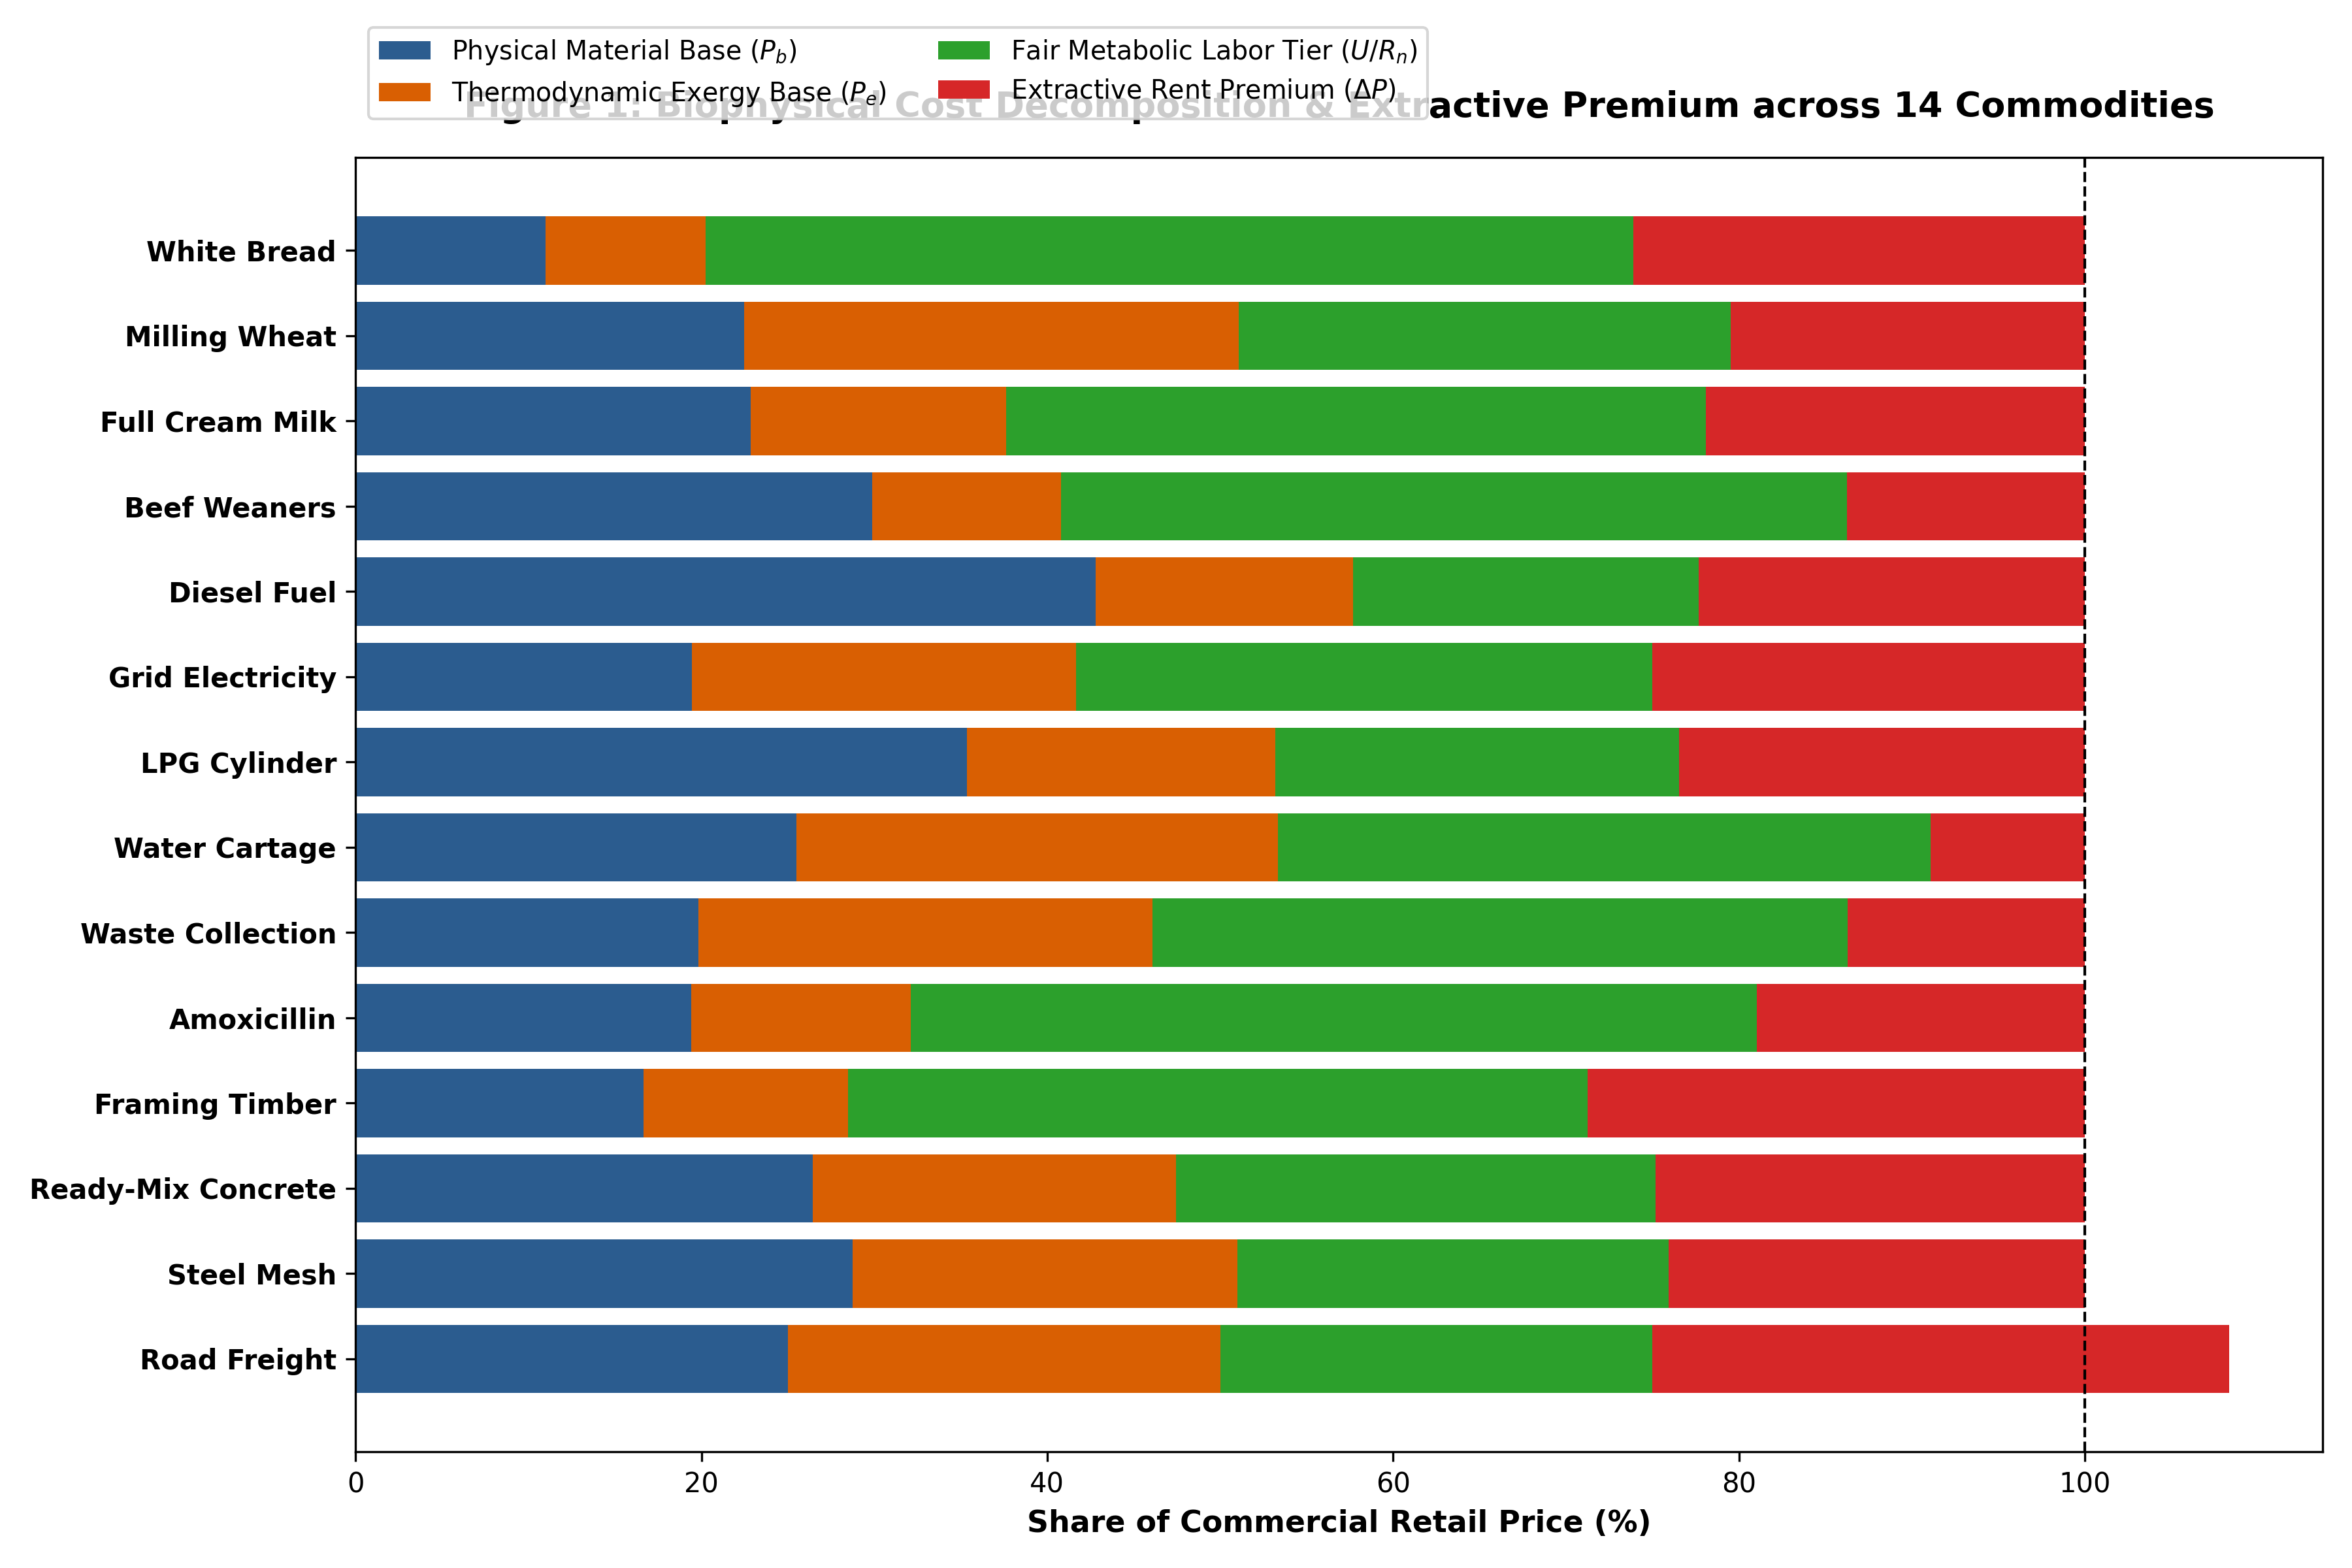
\includegraphics[width=0.92\textwidth]{figure1_biophysical_breakdown.png}
\caption{Biophysical cost decomposition as a share of observed retail price across 14 commodities, highlighting the extractive rent premium ($\Delta P$).}
\label{fig:fig1}
\end{figure}

\begin{figure}[H]
\centering
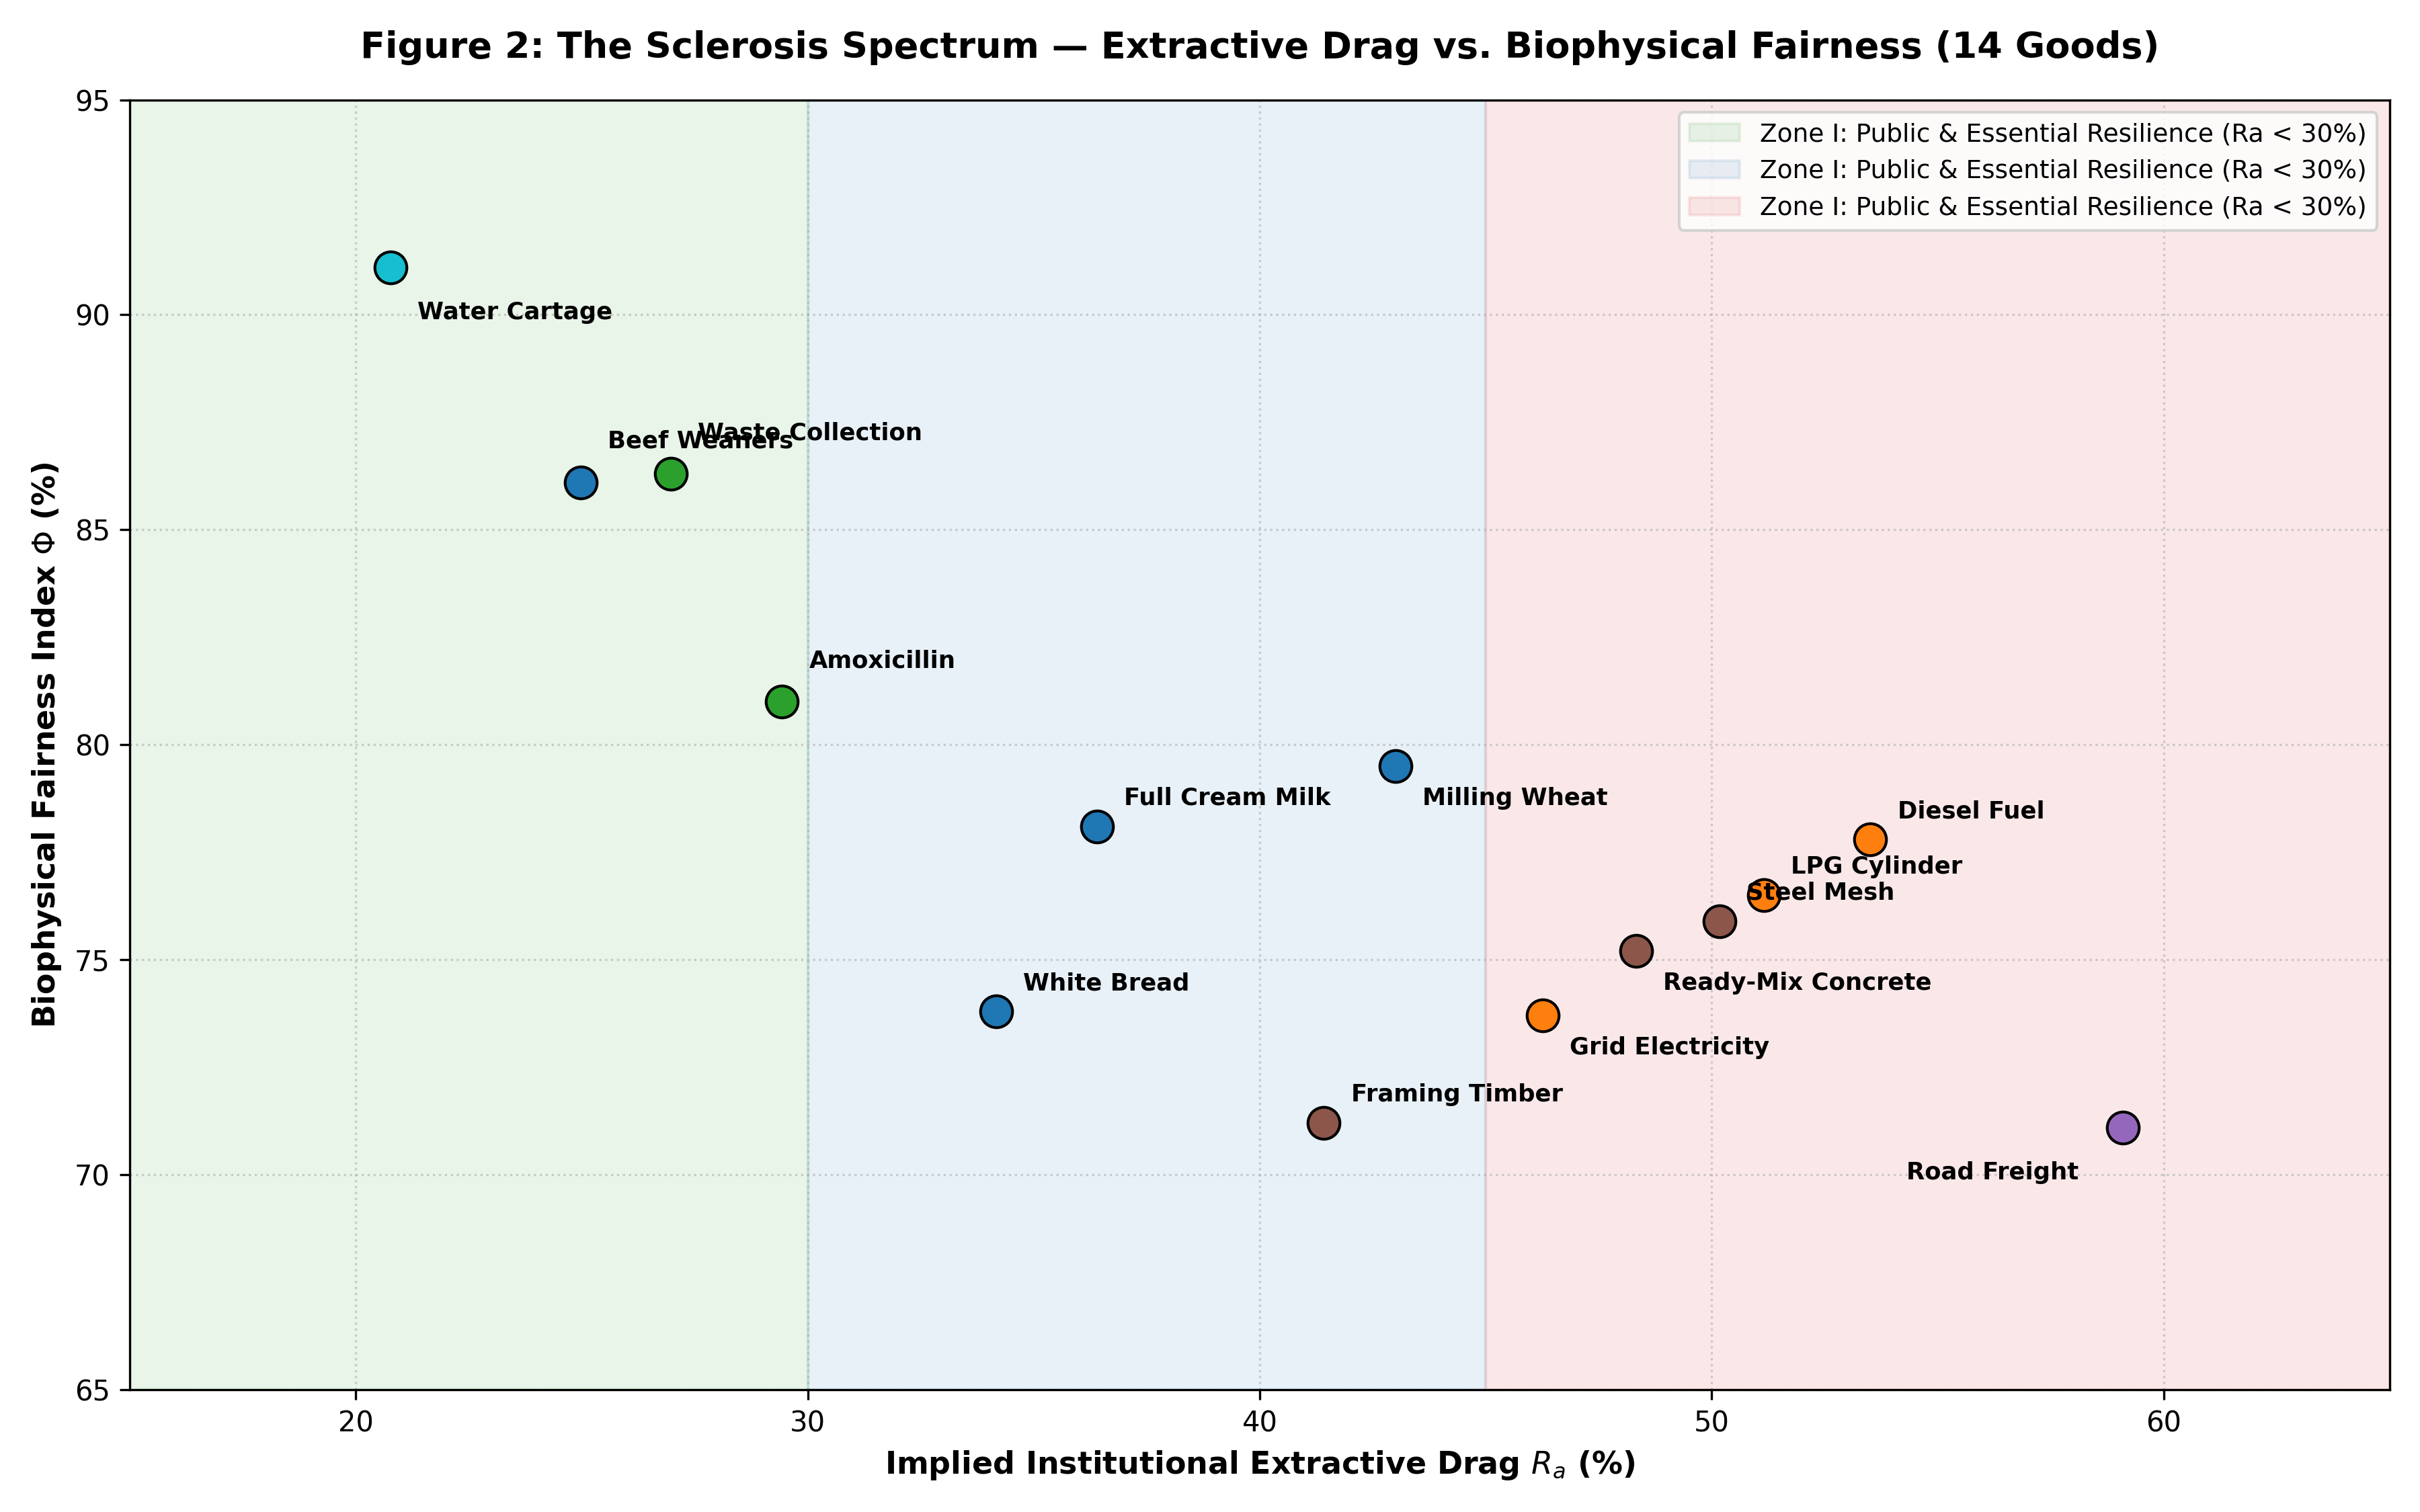
\includegraphics[width=0.92\textwidth]{figure2_sclerosis_spectrum.png}
\caption{The Sclerosis Spectrum: Implied institutional extractive drag ($R_a$) versus Biophysical Fairness Index ($\Phi$).}
\label{fig:fig2}
\end{figure}

\section{Macroeconomic Structural Synthesis: The Three Extraction Tiers}
The empirical results reveal three distinct institutional pricing regimes in the real economy:
\begin{enumerate}
    \item \textbf{Tier I: Public, Clinical \& Producer Resilience (Water Cartage, Waste Collection, Beef Weaners, Antibiotics):} Characterized by high Fairness Indices (81.0\%--91.1\%) and low extractive drag ($R_a = 20.8\%$--$29.4\%$). Pricing directly tracks thermodynamic exergy ($P_e$) and operator/clinical difficulty ($U$), providing an uncorrupted biophysical baseline.
    \item \textbf{Tier II: Agricultural Subsistence Staples (Bread, Wheat, Milk):} Characterized by intermediate drag ($R_a = 34.2\%$--$43.0\%$) and moderate fairness (73.8\%--79.5\%). Supermarket duopoly distribution tollbooths and processor oligopsonies capture between 34\% and 43\% of retail value, squeezing farmgate returns below reproduction costs.
    \item \textbf{Tier III: Corporate and Monopolistic Enclosures (Diesel Fuel, Steel Mesh, Ready-Mix Concrete, Grid Electricity, Structural Timber, Road Freight):} Characterized by severe extractive drag ($R_a = 41.4\%$--$59.1\%$) and compressed Fairness Indices (71.1\%--77.8\%). Across housing construction materials (Timber, Concrete, Steel), unearned distributor rents and oligopolistic markups account for over 45\% of total material costs. Road freight logistics imposes an unprecedented 59.1\% broker toll that cascades inflation into every downstream good.
\end{enumerate}

\section{Policy Implications \& Regulatory Forensics}
\begin{enumerate}
    \item \textbf{Objective Pricing Benchmarks (RRP/D):} By replacing opaque corporate ``cost-plus'' claims with the UPE biophysical difficulty standard, regulatory authorities (such as the ACCC) can enforce price gouging caps anchored directly in physical difficulty.
    \item \textbf{Sovereign Mutual Credit \& Strategic Buffer Reserves:} Eliminating usurious working capital interest charges via Sovereign Mutual Credit Unions (SMCU) and establishing municipal buffer stocks collapses $R_a \to 0.02$, returning retail prices to their fair RRP/D baselines \citep{godley2007monetary, hamilton2026vpe49}.
    \item \textbf{Decoupling from Speculative Indices:} The UPE proves that essential subsistence goods should never be priced via speculative financial exchanges (e.g., CME wheat futures or global oil benchmarks), but rather via their local biophysical reproduction costs.
\end{enumerate}

\section{Conclusion}
This empirical case study demonstrates that the Universal Price Equation is not an abstract theoretical ideal, but an operational auditing instrument capable of diagnosing real-world supply chain sclerosis. By establishing that between 20\% and 59\% of Australian retail prices consist of unearned institutional rents, Value Physics provides a rigorous physical foundation for post-neoclassical economic reform.

\section*{Author Epistemic Statement \& AI Disclosure}
The conceptual ontology, foundational equations, and analytical architecture of the Universal Price Equation (UPE) and Value Physics represent the original intellectual work of Jarrod Lyndsay Hamilton. The author holds no formal academic credentials in economics; theoretical connections were established through self-directed study. Due to memory impairments, the author may not actively retain specific textual details or citations from the research process; readers are encouraged to evaluate the mathematical mechanics, computational solvers, and empirical calibrations directly on their own intrinsic merits. AI tooling (Google Gemini / Gemini Spark) was utilized under the author's direct guidance for computational implementation, code verification, and \LaTeX\ formatting.

\section*{CRediT Authorship Contribution Statement}
\textbf{Jarrod Lyndsay Hamilton:} Conceptualization, Methodology, Formal Analysis, Software, Investigation, Data Curation, Writing -- Original Draft, Visualization.

\section*{Declaration of Competing Interest}
The author declares that he has no known competing financial interests or personal relationships that could have appeared to influence the work reported in this paper.

\section*{Data Availability}
All simulation scripts and calibration datasets are publicly available in the open-source repository \citep{hamilton2026vpe49}.

\bibliographystyle{elsarticle-harv}
\bibliography{references_vpe55}

\end{document}
